% README figure: the method as a block diagram (left) and Fig. 1 of the paper (right).
% Build from this folder:
%   pdflatex readme_figure.tex && pdftoppm -r 200 -png -singlefile readme_figure.pdf ../../reach_avoid_mpc
\documentclass[border=8pt]{standalone}
\usepackage{newtxtext, newtxmath}
\usepackage{bm, amsmath}
\usepackage{tikz}
\usetikzlibrary{arrows.meta, decorations.markings}
% palette of the paper (TAC/root.tex)
\definecolor{setfill}{HTML}{E6F2FF}  \definecolor{setline}{HTML}{2166AC}
\definecolor{termfill}{HTML}{C9DCF0} \definecolor{tgtfill}{HTML}{FEE0D2}
\definecolor{tgtline}{HTML}{D6604D}  \definecolor{obsfill}{HTML}{E6E6E6}
\definecolor{obsline}{HTML}{A6A6A6}  \definecolor{ours}{HTML}{8856A7}
\definecolor{start}{HTML}{FF8C00}    \definecolor{endmark}{HTML}{1A984F}
\tikzset{axis/.style={-{Latex[length=2.2mm, width=1.6mm]}, line width=0.6pt, black}}
\begin{document}
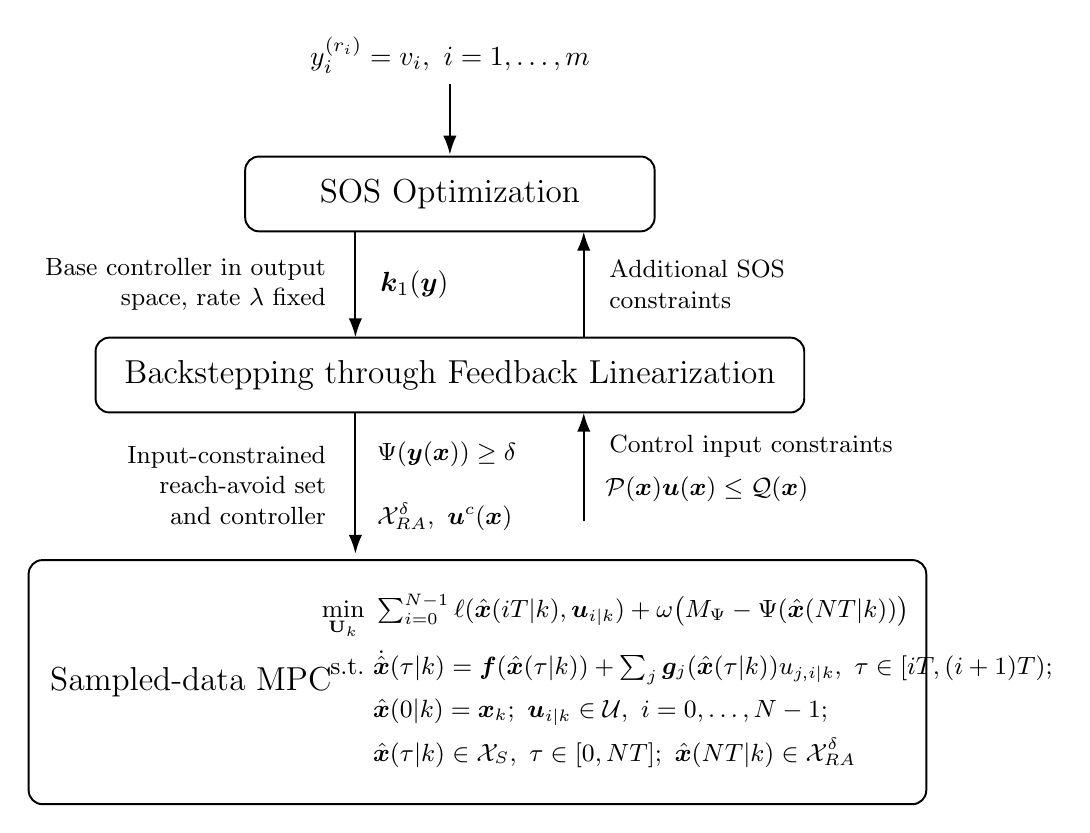
\begin{tikzpicture}[baseline=(current bounding box.center),
    blk/.style={draw, rounded corners=5pt, line width=0.7pt, minimum height=0.95cm, align=center, font=\large},
    arr/.style={-{Latex[length=2.4mm, width=1.7mm]}, line width=0.7pt},
    noter/.style={font=\small, align=right, anchor=east},
    notel/.style={font=\small, align=left, anchor=west}]
    % normal form entering the SOS program
    \draw[arr] (0,9.45) node[above] {$y_i^{(r_i)} = v_i, \ i = 1, \dots, m$} -- (0,8.55);
    \node[blk, minimum width=5.2cm] (sos) at (0,8.05) {SOS Optimization};
    \node[blk, minimum width=9.0cm] (bs) at (0,5.75) {Backstepping through Feedback Linearization};
    % k1 down, additional constraints up
    \draw[arr] (-1.2,7.57) -- (-1.2,6.23);
    \node at (-0.45,6.9) {$\bm{k}_1(\bm{y})$};
    \node[noter] at (-1.45,6.9) {Base controller in output\\space, rate $\lambda$ fixed};
    \draw[arr] (1.7,6.23) -- (1.7,7.57);
    \node[notel] at (1.9,6.9) {Additional SOS\\constraints};
    % reach-avoid set down, input constraints up
    \draw[arr] (-1.2,5.27) -- (-1.2,3.48);
    \node[notel] at (-1.05,4.75) {$\Psi(\bm{y}(\bm{x})) \geq \delta$};
    \node[notel] at (-1.05,3.95) {$\mathcal{X}_{RA}^{\delta}, \ \bm{u}^c(\bm{x})$};
    \node[noter] at (-1.45,4.35) {Input-constrained\\reach-avoid set\\and controller};
    \draw[arr] (1.7,3.9) -- (1.7,5.27);
    \node[notel] at (1.9,4.85) {Control input constraints};
    \node[notel] at (1.85,4.3) {$\mathcal{P}(\bm{x})\bm{u}(\bm{x}) \leq \mathcal{Q}(\bm{x})$};
    % sampled-data MPC
    \node[blk, minimum width=11.4cm, minimum height=3.1cm] (mpc) at (0.35,1.85) {};
    \node[font=\large, anchor=west] at (-5.2,1.85) {Sampled-data MPC};
    \node[anchor=west, font=\small] at (-1.75,1.85) {$\begin{aligned}
        \min_{\mathbf{U}_k} \ & \textstyle\sum_{i=0}^{N-1} \ell(\hat{\bm{x}}(iT|k), \bm{u}_{i|k})
            + \omega\big(M_\Psi - \Psi(\hat{\bm{x}}(NT|k))\big) \\
        \text{s.t.} \ & \dot{\hat{\bm{x}}}(\tau|k) = \bm{f}(\hat{\bm{x}}(\tau|k))
            + \textstyle\sum_{j} \bm{g}_j(\hat{\bm{x}}(\tau|k)) u_{j,i|k}, \ \tau \in [iT, (i+1)T); \\
        & \hat{\bm{x}}(0|k) = \bm{x}_k; \ \bm{u}_{i|k} \in \mathcal{U}, \ i = 0, \dots, N-1; \\
        & \hat{\bm{x}}(\tau|k) \in \mathcal{X}_S, \ \tau \in [0, NT]; \ \hat{\bm{x}}(NT|k) \in \mathcal{X}_{RA}^{\delta}
    \end{aligned}$};
\end{tikzpicture}\hspace{1.2cm}%
% Right panel of the README figure: copy of Fig. 1 of the paper (TAC/figs/fig_pipeline.tikz)
% with descriptive labels and a larger scale; built by readme_figure.tex.
% Top view of a car as a TikZ pic, for Fig. 1 (figs/fig_pipeline.tikz).
% Traced from figs/car_topview.svg (Openclipart, public domain) and reduced
% to what stays legible at about 1 cm: the body, the tyres, the mirrors and
% the outlines of the four windows, which are left uncoloured. The car is
% centred at the origin, points along +x and is 1 unit long, so `scale'
% sets its length in cm. Colours refer to the palette defined in root.tex;
% change the `car ...' styles below to recolour it, for instance
% `car window/.style={car line, fill=white}' for filled windows.
\tikzset{
    car line/.style={draw=ours!65!black, line width=0.5pt, line join=round},
    car body/.style={car line, fill=ours!35},
    car window/.style={car line, line width=0.4pt, fill=white},
    car tyre/.style={fill=black!70},
    pics/car/.style={code={
        % tyres
        \path[car tyre]
        (-0.289,0.196) -- (-0.289,0.182)
            .. controls (-0.289,0.176) and (-0.294,0.171) .. (-0.300,0.171)
            -- (-0.378,0.171)
            .. controls (-0.384,0.171) and (-0.389,0.176) .. (-0.389,0.182)
            -- (-0.389,0.196)
            .. controls (-0.389,0.202) and (-0.384,0.207) .. (-0.378,0.207)
            -- (-0.300,0.207)
            .. controls (-0.294,0.207) and (-0.289,0.202) .. (-0.289,0.196)
            -- cycle;
        \path[car tyre]
        (-0.277,-0.178) -- (-0.277,-0.191)
            .. controls (-0.277,-0.197) and (-0.281,-0.202) .. (-0.288,-0.202)
            -- (-0.365,-0.202)
            .. controls (-0.371,-0.202) and (-0.376,-0.197) .. (-0.376,-0.191)
            -- (-0.376,-0.178)
            .. controls (-0.376,-0.172) and (-0.371,-0.167) .. (-0.365,-0.167)
            -- (-0.288,-0.167)
            .. controls (-0.281,-0.167) and (-0.277,-0.172) .. (-0.277,-0.178)
            -- cycle;
        \path[car tyre]
        (0.376,-0.187) -- (0.376,-0.201)
            .. controls (0.376,-0.207) and (0.371,-0.212) .. (0.365,-0.212)
            -- (0.287,-0.212)
            .. controls (0.281,-0.212) and (0.276,-0.207) .. (0.276,-0.201)
            -- (0.276,-0.187)
            .. controls (0.276,-0.181) and (0.281,-0.177) .. (0.287,-0.177)
            -- (0.365,-0.177)
            .. controls (0.371,-0.177) and (0.376,-0.181) .. (0.376,-0.187)
            -- cycle;
        \path[car tyre]
        (0.372,0.205) -- (0.372,0.192)
            .. controls (0.372,0.186) and (0.367,0.181) .. (0.361,0.181)
            -- (0.283,0.181)
            .. controls (0.277,0.181) and (0.272,0.186) .. (0.272,0.192)
            -- (0.272,0.205)
            .. controls (0.272,0.211) and (0.277,0.216) .. (0.283,0.216)
            -- (0.361,0.216)
            .. controls (0.367,0.216) and (0.372,0.211) .. (0.372,0.205)
            -- cycle;
        % body
        \path[car body]
        (-0.492,0.001)
            .. controls (-0.495,0.144) and (-0.469,0.166) .. (-0.465,0.187)
            .. controls (-0.416,0.208) and (-0.002,0.212) .. (0.032,0.200)
            .. controls (0.109,0.190) and (0.122,0.206) .. (0.214,0.211)
            .. controls (0.322,0.220) and (0.262,0.198) .. (0.372,0.216)
            .. controls (0.486,0.189) and (0.488,0.241) .. (0.499,0.003)
            .. controls (0.496,-0.215) and (0.486,-0.185) .. (0.372,-0.212)
            .. controls (0.262,-0.194) and (0.322,-0.215) .. (0.214,-0.206)
            .. controls (0.122,-0.202) and (0.109,-0.186) .. (0.032,-0.195)
            .. controls (-0.002,-0.208) and (-0.416,-0.204) .. (-0.465,-0.183)
            .. controls (-0.484,-0.150) and (-0.492,-0.062) .. (-0.492,0.001)
            -- cycle;
        % window frames
        \path[car window]
        (0.170,0.170)
            .. controls (0.170,0.170) and (0.202,0.089) .. (0.203,-0.001)
            .. controls (0.203,-0.082) and (0.191,-0.119) .. (0.173,-0.169)
            .. controls (0.116,-0.163) and (0.063,-0.157) .. (0.045,-0.142)
            .. controls (0.078,-0.004) and (0.078,0.005) .. (0.045,0.143)
            .. controls (0.063,0.146) and (0.167,0.173) .. (0.170,0.170)
            -- cycle;
        \path[car window]
        (-0.180,0.125)
            .. controls (-0.252,0.140) and (-0.389,0.152) .. (-0.389,0.152)
            .. controls (-0.410,0.128) and (-0.419,0.005) .. (-0.419,0.002)
            .. controls (-0.419,-0.007) and (-0.410,-0.130) .. (-0.380,-0.151)
            .. controls (-0.362,-0.151) and (-0.234,-0.139) .. (-0.177,-0.127)
            .. controls (-0.192,-0.022) and (-0.186,0.119) .. (-0.180,0.125)
            -- cycle;
        \path[car window]
        (0.125,0.173)
            .. controls (0.125,0.173) and (0.030,0.152) .. (0.030,0.152)
            .. controls (0.030,0.152) and (-0.150,0.152) .. (-0.153,0.155)
            .. controls (-0.156,0.158) and (-0.207,0.182) .. (-0.207,0.182)
            .. controls (-0.207,0.182) and (0.119,0.176) .. (0.125,0.173)
            -- cycle;
        \path[car window]
        (0.131,-0.175)
            .. controls (0.131,-0.175) and (0.036,-0.154) .. (0.036,-0.154)
            .. controls (0.036,-0.154) and (-0.144,-0.154) .. (-0.147,-0.157)
            .. controls (-0.150,-0.160) and (-0.201,-0.183) .. (-0.201,-0.183)
            .. controls (-0.201,-0.183) and (0.125,-0.178) .. (0.131,-0.175)
            -- cycle;
        % mirrors
        \path[car body]
        (0.146,-0.180) -- (0.143,-0.216)
            .. controls (0.143,-0.216) and (0.125,-0.234) .. (0.117,-0.222)
            .. controls (0.108,-0.210) and (0.120,-0.180) .. (0.120,-0.180)
            -- (0.146,-0.180) -- cycle;
        \path[car body]
        (0.140,0.180) -- (0.137,0.216)
            .. controls (0.137,0.216) and (0.119,0.234) .. (0.111,0.222)
            .. controls (0.102,0.210) and (0.114,0.180) .. (0.114,0.180)
            -- (0.140,0.180) -- cycle;
    }},
}

\begin{tikzpicture}[x=1cm, y=1cm, scale=1.3, baseline=(current bounding box.center),
    safe/.style={setline, thick, fill=setfill},
    term/.style={setline, thick, dashed, fill=termfill},
    tgt/.style={tgtline, thick, fill=tgtfill},
    obs/.style={draw=obsline, thick, fill=obsfill, line join=round},
    mpc/.style={ours, thick},
    uc/.style={ours, thick, dashed, -{Latex[length=2.2mm, width=1.6mm]}},
    sample/.style={fill=black!75},
    lbl/.style={font=\small},
    car at/.store in=\carpos, car at=0.68,
    car size/.store in=\carsize, car size=1.0]

    % axes
    \draw[axis] (-0.25,0) -- (6.45,0);
    \draw[axis] (0,-0.25) -- (0,6.45);

    % unsafe regions
    \draw[obs] (3.24,6.01) -- (2.84,5.39) -- (3.22,4.88) -- (4.82,5.51)
        -- (6.02,5.31) -- (5.79,6.20) -- cycle;
    \draw[obs] (0.34,4.03) -- (1.07,2.65) -- (0.18,1.49) -- cycle;

    % safe set X_S
    \draw[safe] (0.69,5.98) .. controls (0.30,5.77) and (0.28,4.88) .. (0.63,4.43)
        .. controls (1.10,3.81) and (1.41,2.71) .. (1.36,2.38)
        .. controls (1.31,2.05) and (0.32,1.79) .. (0.80,1.31)
        .. controls (1.58,0.52) and (2.78,0.66) .. (3.15,0.71)
        .. controls (4.51,0.87) and (5.31,1.78) .. (5.60,2.11)
        .. controls (5.86,2.41) and (5.92,2.72) .. (6.03,3.27)
        .. controls (6.07,3.50) and (6.10,3.77) .. (5.76,4.83)
        .. controls (5.56,5.45) and (3.00,4.49) .. (2.67,4.64)
        .. controls (2.09,4.91) and (3.13,5.85) .. (2.69,6.22)
        .. controls (2.50,6.38) and (1.53,6.45) .. cycle;

    % terminal set X_RA^delta
    \draw[term] (3.20,4.20) .. controls (2.88,4.02) and (1.61,3.49) .. (1.78,2.95)
        .. controls (1.96,2.38) and (1.91,2.26) .. (1.90,1.98)
        .. controls (1.89,1.66) and (1.35,1.43) .. (1.80,1.27)
        .. controls (2.68,0.95) and (2.85,0.87) .. (3.16,0.90)
        .. controls (4.29,1.04) and (4.56,1.31) .. (4.86,1.53)
        .. controls (5.14,1.73) and (5.78,2.51) .. (5.87,2.97)
        .. controls (5.90,3.16) and (5.52,3.21) .. (5.75,3.86)
        .. controls (5.93,4.37) and (5.45,4.93) .. (5.15,4.88)
        .. controls (4.53,4.78) and (4.84,3.95) .. (4.27,3.82)
        .. controls (3.85,3.72) and (3.90,4.59) .. cycle;

    % target set X_T, partly outside X_S
    \draw[tgt] (5.79,1.46) .. controls (5.69,1.52) and (5.49,2.34) .. (5.17,2.34)
        .. controls (4.78,2.34) and (4.51,2.14) .. (4.29,1.98)
        .. controls (4.08,1.82) and (3.86,1.66) .. (3.75,1.35)
        .. controls (3.71,1.27) and (3.60,0.95) .. (3.75,0.59)
        .. controls (3.91,0.19) and (4.83,-0.03) .. (4.52,0.27)
        .. controls (3.98,0.77) and (5.03,0.67) .. (5.35,0.38)
        .. controls (5.64,0.12) and (6.12,0.24) .. (6.26,0.69)
        .. controls (6.31,0.85) and (6.34,1.51) .. (6.20,1.78)
        .. controls (6.11,1.97) and (5.92,1.38) .. cycle;

    % terminal controller inside X_RA^delta, into X_T
    \draw[uc] (2.84,4.03) .. controls (2.85,3.97) and (2.34,3.37) .. (2.58,3.29)
        .. controls (2.80,3.20) and (3.31,3.27) .. (3.62,3.42)
        .. controls (3.85,3.52) and (4.13,3.34) .. (4.31,3.16)
        .. controls (4.47,3.00) and (4.52,1.94) .. (4.51,1.59);

    % sampled-data MPC from x_0 to X_RA^delta, with sampling instants and car
    \coordinate (x0) at (2.37,5.98);
    \coordinate (xN) at (2.84,4.03);
    \draw[mpc,
        postaction={decorate, decoration={markings,
            % sampling instants, positions in increasing order, kept clear of the car
            mark=at position 0.18 with {\fill[sample] (0,0) circle (1.3pt);},
            mark=at position 0.36 with {\fill[sample] (0,0) circle (1.3pt);},
            mark=at position 0.50 with {\fill[sample] (0,0) circle (1.3pt);},
            mark=at position 0.88 with {\fill[sample] (0,0) circle (1.3pt);}}},
        postaction={decorate, decoration={markings,
            mark=at position \carpos with {\pic[scale=\carsize] {car};}}}]
        (x0) .. controls (2.08,5.95) and (1.58,5.82) .. (1.62,5.54)
        .. controls (1.69,5.06) and (1.24,4.78) .. (1.25,4.33)
        .. controls (1.27,3.82) and (2.94,4.36) .. (xN);
    \fill[sample] (xN) circle (1.3pt);
    \fill[start] (x0) circle (2.3pt);

    % labels
    \node[lbl, below=1pt, align=center] at (x0) {$\bm{x}_0$};
    \node[lbl, align=center] at (0.92,5.25) {Safe set\\$\mathcal{X}_S$};
    \node[lbl, align=center] at (2.75,1.9) {Terminal set\\$\mathcal{X}_{RA}^{\delta}$};
    \node[lbl, align=center] at (5.35,1.05) {Target set\\$\mathcal{X}_T$};
    \node[lbl, anchor=west] at (0.15,0.32) {State space $\mathcal{X}$};
\end{tikzpicture}

\end{document}
